Barometer er ett instrument eller en elektrisk sensor som måler lufttrykk. 
Prosjektet tar for seg barometer for å beregne høyde, i prosjektet blir 
elektrisk sensor som sensoren i figur \ref{fig:bme280} brukt. Luftrykket på 
jorda minker ved økning i høyde, denne endringen i luftrykket kan bli brukt for å estimere høyde. 
Luftrykket kan endret av lokale trykkvariasjoner på jorda. Her har vær, klima, 
tidevann og temperatur noe å si. Ved bruk av barometer for høyde 
beregninger er det derfor nødvendig å kalibrere barometeret først. Bruk av barometer for høydeangivelse 
innendørs kan gi problemer med uønskede trykkendringer. Her kan åpning av dører eller 
bruk av ventilasjonssystemer skape store trykkforskjeller.
\parencite{Gron2021piezo}

\begin{figure}[htp]
    \centering
    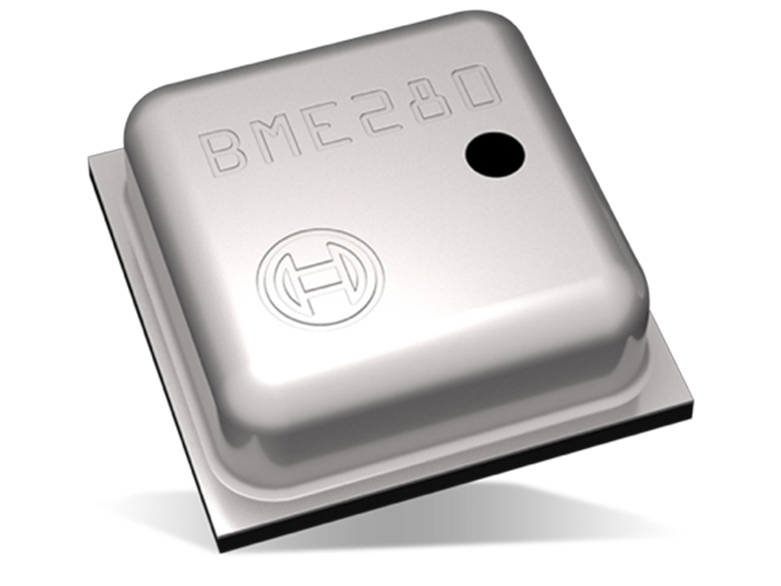
\includegraphics[width=0.5\columnwidth]{figures/bme280}
    \caption{BME280. \parencite{Bosch}}
    \label{fig:bme280}
\end{figure}